\chapter{Topic: Multiple Inheritance}

\begin{aside}
Material from the remainder of the term, not covered in the original lecture
notes.
\end{aside}

\section{Basics}
A class can inherit from more than one class:
\begin{lstlisting}[style=cpp]
class A1 {
  public:
    int a;
};
class A2 {
  public:
    int b;
};
class B : public A1, public A2 {
  public:
    int c;
};

B obj;
obj.a; obj.b; obj.c;    // B has all three fields
\end{lstlisting}

\begin{center}
\begin{tikzpicture}[cls/.style={draw, minimum width=16mm, minimum height=8mm}]
\node[cls] (a1) {A1};
\node[cls, right=20mm of a1] (a2) {A2};
\node[cls, below=12mm of $(a1)!0.5!(a2)$] (b) {B};
\draw[-{Triangle[open,length=3mm,width=3mm]}] (b.north) -- (a1.south east);
\draw[-{Triangle[open,length=3mm,width=3mm]}] (b.north) -- (a2.south west);
\end{tikzpicture}
\end{center}

\section{Ambiguity}
Problems arise when the base classes have members with the same name:
\begin{lstlisting}[style=cpp]
class A1 { public: void foo() { cout << "A1::foo"; } };
class A2 { public: void foo() { cout << "A2::foo"; } };
class B : public A1, public A2 {};

B b;
b.foo();       // error: ambiguous
b.A1::foo();   // OK: say which one
b.A2::foo();   // OK
\end{lstlisting}

\section{The Diamond Problem}
Suppose both bases themselves inherit from a common class:
\begin{lstlisting}[style=cpp]
class A { public: int a; };
class B : public A { ... };
class C : public A { ... };
class D : public B, public C { ... };

D d;
d.a;           // error: ambiguous -- which a?
\end{lstlisting}

\begin{center}
\begin{tikzpicture}[cls/.style={draw, minimum width=14mm, minimum height=8mm}]
\node[cls] (a) {A};
\node[cls, below left=10mm and 8mm of a] (b) {B};
\node[cls, below right=10mm and 8mm of a] (c) {C};
\node[cls, below right=10mm and 8mm of b] (d) {D};
\draw[-{Triangle[open,length=3mm,width=3mm]}] (b) -- (a);
\draw[-{Triangle[open,length=3mm,width=3mm]}] (c) -- (a);
\draw[-{Triangle[open,length=3mm,width=3mm]}] (d) -- (b);
\draw[-{Triangle[open,length=3mm,width=3mm]}] (d) -- (c);
\end{tikzpicture}
\end{center}

By default, a \code{D} contains \emph{two} A parts: one inside its B part and
one inside its C part. So \code{d.a} is ambiguous; we would have to say
\code{d.B::a} or \code{d.C::a}. Usually that isn't what we want: there should be
only one A in a D.
\begin{center}
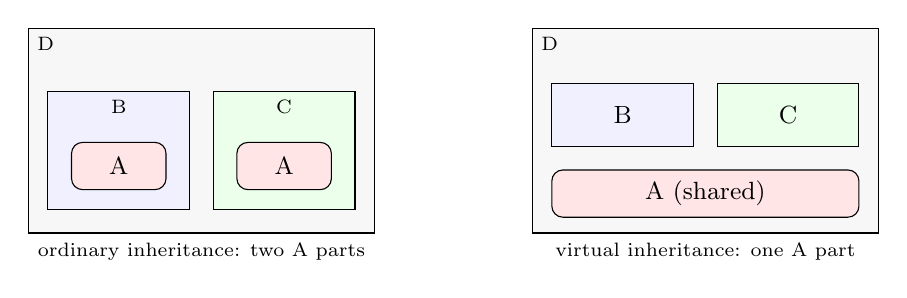
\begin{tikzpicture}[font=\small,p/.style={draw,rounded corners,minimum width=1.6cm,minimum height=0.6cm}]
  \node[draw,fill=gray!6,minimum width=4.4cm,minimum height=2.6cm] (d) at (0,0) {};
  \node[font=\scriptsize,anchor=north west] at (d.north west) {D};
  \node[draw,fill=blue!6,minimum width=1.8cm,minimum height=1.5cm] (b) at (-1.05,-0.25) {};
  \node[font=\scriptsize,anchor=north] at (b.north) {B};
  \node[p,fill=red!10,minimum width=1.2cm] at (-1.05,-0.45) {A};
  \node[draw,fill=green!8,minimum width=1.8cm,minimum height=1.5cm] (c) at (1.05,-0.25) {};
  \node[font=\scriptsize,anchor=north] at (c.north) {C};
  \node[p,fill=red!10,minimum width=1.2cm] at (1.05,-0.45) {A};
  \node[font=\scriptsize,anchor=north] at (d.south) {ordinary inheritance: two A parts};
  \begin{scope}[xshift=6.4cm]
  \node[draw,fill=gray!6,minimum width=4.4cm,minimum height=2.6cm] (d) at (0,0) {};
  \node[font=\scriptsize,anchor=north west] at (d.north west) {D};
  \node[draw,fill=blue!6,minimum width=1.8cm,minimum height=0.8cm] at (-1.05,0.2) {B};
  \node[draw,fill=green!8,minimum width=1.8cm,minimum height=0.8cm] at (1.05,0.2) {C};
  \node[p,fill=red!10,minimum width=3.9cm] at (0,-0.8) {A (shared)};
  \node[font=\scriptsize,anchor=north] at (d.south) {virtual inheritance: one A part};
  \end{scope}
\end{tikzpicture}
\end{center}

\subsection{Virtual Inheritance}
Make A a \textbf{virtual base class}:
\begin{lstlisting}[style=cpp]
class B : virtual public A { ... };
class C : virtual public A { ... };
class D : public B, public C { ... };

D d;
d.a;           // OK: there is only one A part
\end{lstlisting}
Example from the standard library: \code{iostream} inherits from both
\code{istream} and \code{ostream}, which both virtually inherit from
\code{ios\_base}/\code{ios} (the shared stream state).
\begin{center}
\begin{tikzpicture}[cls/.style={draw,fill=blue!4,minimum height=7mm,font=\ttfamily\small},
  inh/.style={-{Triangle[open,length=3mm,width=3mm]}}]
  \node[cls] (ios) at (0,0) {ios};
  \node[cls] (is) at (-1.8,-1.4) {istream};
  \node[cls] (os) at (1.8,-1.4) {ostream};
  \node[cls] (io) at (0,-2.8) {iostream};
  \draw[inh] (is) -- node[left,font=\scriptsize\rmfamily]{virtual} (ios);
  \draw[inh] (os) -- node[right,font=\scriptsize\rmfamily]{virtual} (ios);
  \draw[inh] (io) -- (is); \draw[inh] (io) -- (os);
\end{tikzpicture}
\end{center}

\paragraph{Construction.} With virtual inheritance, B and C must not both
construct the single shared A part. The rule is that the \emph{most derived}
class constructs the virtual base directly:
\begin{lstlisting}[style=cpp]
D::D(...) : A{...}, B{...}, C{...} {}   // D calls A's ctor itself;
                                        // B's and C's calls to A{...} are ignored
\end{lstlisting}

\section{Object Layout}
Without virtual inheritance, a D looks like
\begin{center}
\begin{tabular}{|c|}
\hline
vptr \\ \hline
A fields (B's copy) \\ \hline
B fields \\ \hline
vptr \\ \hline
A fields (C's copy) \\ \hline
C fields \\ \hline
D fields \\ \hline
\end{tabular}
\end{center}
A pointer to a D works as a pointer to its B part (same start address), but
\emph{not} directly as a pointer to its C part, which starts further in. So
converting a \code{D*} to a \code{C*} must \emph{adjust} the pointer's value:
\begin{lstlisting}[style=cpp]
D *pd = new D;
C *pc = pd;                       // compiler adds the offset of the C part
cout << (void*)pd << " " << (void*)pc;   // different addresses!
\end{lstlisting}
\begin{center}
\begin{tikzpicture}[>=Stealth,f/.style={draw,minimum width=3.2cm,minimum height=5.5mm,font=\small}]
  \node[f,fill=gray!10] (v1) at (0,0) {vptr};
  \node[f,fill=red!10,below=0mm of v1] (a1) {A fields (B's copy)};
  \node[f,fill=blue!6,below=0mm of a1] (b) {B fields};
  \node[f,fill=gray!10,below=0mm of b] (v2) {vptr};
  \node[f,fill=red!10,below=0mm of v2] (a2) {A fields (C's copy)};
  \node[f,fill=green!8,below=0mm of a2] (c) {C fields};
  \node[f,fill=orange!12,below=0mm of c] (d) {D fields};
  \draw[<-] (v1.west) -- ++(-1.2,0) node[left,font=\scriptsize]{\code{pd}, and \code{B*}};
  \draw[<-] (v2.west) -- ++(-1.2,0) node[left,font=\scriptsize]{\code{pc}};
  \draw[decorate,decoration={brace,amplitude=4pt}] ([xshift=3pt]v1.north east) -- ([xshift=3pt]b.south east) node[midway,right=6pt,font=\scriptsize]{B part};
  \draw[decorate,decoration={brace,amplitude=4pt}] ([xshift=3pt]v2.north east) -- ([xshift=3pt]c.south east) node[midway,right=6pt,font=\scriptsize]{C part};
\end{tikzpicture}

\small Converting \code{D*} to \code{C*} adds the offset of the C part.
\end{center}
\code{static\_cast} and \code{dynamic\_cast} perform this adjustment;
\code{reinterpret\_cast} does not (another reason never to use it for this).

With virtual inheritance, the shared A part is placed at the end of the object,
and its location can differ between a standalone B, a B inside a D, etc. The
vtable stores the offset to the virtual base so code compiled for B can find its
A part at run time:
\begin{center}
\begin{tabular}{|c|}
\hline
vptr (B part) \\ \hline
B fields \\ \hline
vptr (C part) \\ \hline
C fields \\ \hline
D fields \\ \hline
vptr \\ \hline
A fields (shared) \\ \hline
\end{tabular}
\end{center}
This is why accessing members of a virtual base is slightly slower, and why
virtual inheritance should not be used unless the diamond actually arises.

\section{When to Use Multiple Inheritance}
\begin{itemize}
  \item Multiple inheritance of \emph{interfaces} (abstract classes with only
        pure virtual methods, like Java interfaces) is common and safe: e.g.\ a
        class that is both an \code{Observer} and a \code{Subject} (a cell in a
        spreadsheet observes the cells it depends on, and is observed by those
        that depend on it).
  \item Multiple inheritance of \emph{implementations}, especially diamonds, gets
        complicated quickly. Prefer composition when the relationship is not
        clearly is-a for every base.
\end{itemize}

\section*{Summary}
\begin{itemize}
  \item A class may have several base classes; same-named members are ambiguous
        and must be qualified (\code{b.A1::foo()}).
  \item In a diamond, the common base is duplicated unless the inheritance is
        \code{virtual}; the most derived class constructs a virtual base.
  \item Converting a pointer to a non-first base adjusts its address; virtual
        bases are located through the vtable.
  \item Multiple inheritance of interfaces is fine; of implementations, use with
        care.
\end{itemize}
